\chapter{Theoretical framework}

In this chapter we will present the necessary concepts to fully understand the work done. First, we will review general concepts of artificial intelligence (AI), Machine Learning (ML) Image Processing, Object Classification and Object Detection. Second, we will describe the datasets used in this work and finally we will talk about Continual Learning and describe the State-of-the-Art (SOTA) methods.

\section{Artificial Intelligence}

\subsection{Computer Vision}

\subsection{Machine Learning}

\subsection{Vision Transformers}

\subsection{Object Classification}

\subsection{Object Detection}

\section{Image Datasets}
Several image datasets were utilized in the course of this work. A detailed description of each dataset is provided below.

\subsection{ImageNet}

ImageNet \cite{imagenet} is a large-scale visual database widely used in computer vision research. It is organized according to the WordNet hierarchy and provides annotated, high-resolution images across 1,000 object classes, making it a standard benchmark for large-scale image classification. The dataset contains over 1.2 million training images, 50,000 validation images, and 100,000 test images, covering a broad diversity of real-world objects. Its scale, diversity, and hierarchical structure have established ImageNet as a cornerstone resource for evaluating and advancing machine learning models in image recognition and related tasks.

\subsubsection{ImageNetR}
ImageNet-R (ImageNet-Renditions) \cite{imagenetR} is a dataset derived from ImageNet, consisting of images that depict objects through non-photographic styles such as art, cartoons, graffiti, embroidery, origami, paintings, patterns, sculptures, sketches, tattoos, toys, and video game graphics. It covers 200 ImageNet classes and contains approximately 30,000 images. The dataset was constructed by collecting diverse renditions of ImageNet classes and retaining only those samples that standard models, such as ResNet-50, failed to classify correctly. As a result, ImageNet-R provides a challenging benchmark for evaluating the robustness and generalization of visual recognition models beyond natural images.

\subsubsection{ImageNet21k}

While ImageNet-1K serves as the primary dataset for pretraining deep learning models for computer vision, ImageNet-21K \cite{imagenet21k} offers a much broader and more diverse coverage of visual concepts. It is an extended version of the ImageNet dataset and contains over 14 million annotated images spanning approximately 21,000 semantic classes derived from the WordNet hierarchy. Although historically less utilized due to its size, complexity, and accessibility challenges, recent advances in preprocessing, hierarchical structuring, and training schemes have demonstrated its significant value for pretraining. Models pretrained on ImageNet-21K have shown improved performance and generalization across a wide range of computer vision tasks, including when transferred to more compact architectures such as mobile-oriented networks.

\subsection{CIFAR100}

CIFAR-100 \cite{cifar100} is an image classification dataset that extends the structure of CIFAR-10 to a more fine-grained setting. It consists of 60,000 color images of size 32×32 pixels, divided into 100 classes with 600 images per class. Each class contains 500 training samples and 100 test samples. The classes are grouped into 20 superclasses, providing both a fine label (the specific class) and a coarse label (the superclass). This hierarchical organization allows for evaluating both fine-grained recognition and broader categorization. The dataset includes a wide variety of semantic groups, such as animals (e.g., aquatic mammals, insects, reptiles), objects (e.g., household furniture, vehicles), and natural scenes (e.g., forests, mountains, sea), making it a challenging benchmark for image classification and hierarchical learning tasks.


\subsection{Caltech256}
Caltech-256 \cite{caltech256} is a widely used dataset for object recognition research. It contains 30,607 images distributed across 256 object categories plus an additional ``clutter'' category for background rejection. Each category includes a minimum of 80 images, providing greater balance compared to earlier datasets such as Caltech-101. The images were collected from the web and manually screened to ensure quality, with improvements introduced to avoid artifacts and increase category diversity. Due to its scale and variability, Caltech-256 serves as a challenging benchmark for evaluating classification performance and the generalization ability of visual recognition models.




\section{Continual Learning}
Continual Learning (CL), also known as lifelong learning, constitutes the core focus of this work. It represents a machine learning paradigm designed to handle the progressive acquisition of knowledge from sequences of tasks or data streams over time. In contrast to conventional training approaches, which rely on a fixed dataset and a single training phase, CL emphasizes the ongoing integration of new information while preserving previously learned knowledge. This property is crucial for real-world scenarios where data distributions are non-stationary and environments evolve continuously. The principal challenge lies in mitigating catastrophic forgetting, a phenomenon in which the assimilation of new knowledge leads to the degradation or loss of prior learning \cite{CL}.


\subsection{Elasticity and Plasticity}

A central concept in continual learning is the balance between elasticity and plasticity. Plasticity refers to the ability of a model to adapt rapidly to new information, ensuring that it can effectively learn novel tasks. Elasticity, in contrast, emphasizes stability by preserving the parameters and representations that are crucial for retaining old knowledge \cite{API}. Achieving an appropriate equilibrium between these two properties is known as the stability–plasticity dilemma: models that are overly plastic may forget past tasks, whereas models that are overly elastic may struggle to integrate new knowledge. Successful continual learning methods are therefore designed to optimize this trade-off.

\subsection{Main Paradigms}

As shown in figure \ref{fig:task_vs_class}, two principal paradigms define how continual learning problems are formulated. Task-incremental learning (Task-IL) assumes that the task identity is available during inference \cite{task_il}. In this setting, models can rely on task labels to select the appropriate output head, thereby simplifying the classification problem. Class-incremental learning (Class-IL), on the other hand, does not provide the task identity at test time \cite{masana_class_il}. The model must classify examples among all the classes encountered so far, which makes the problem significantly more challenging. Class-IL is closer to real-world conditions, as systems are rarely informed of which ``task” a new input belongs to during deployment.

\begin{figure} % h=here, t=top, b=bottom, p=page of floats
	\centering
	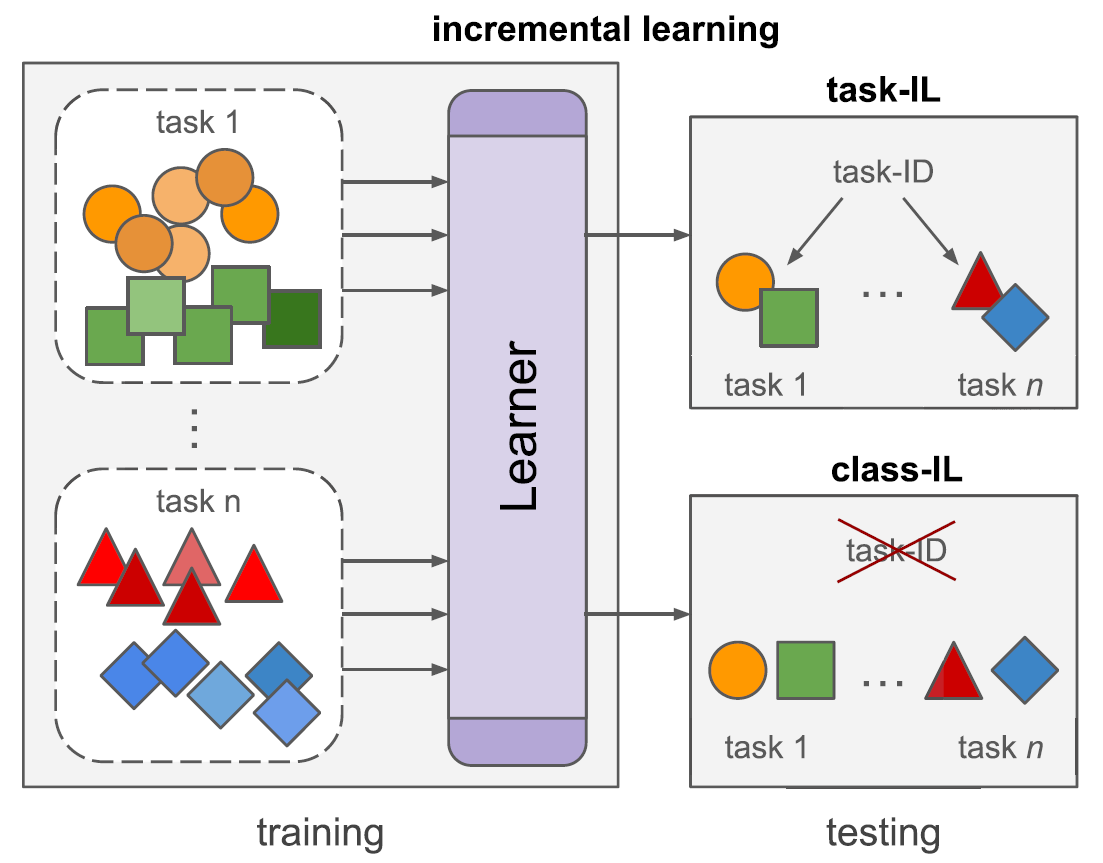
\includegraphics[width=0.5\textwidth]{imagenes/marco/CI_learning_survey_fig1.png} % change path and filename
	\caption{Class and Task Incremental Learning \cite{masana_class_il}.}
	\label{fig:task_vs_class}
\end{figure}


\subsection{Mitigation Strategies}

In this work, the discussion of continual learning strategies is organized into three main categories. The first category comprises rehearsal-based methods, which mitigate forgetting by storing or generating representative samples from previous tasks and replaying them during training. The second category encompasses regularization-based methods, which constrain parameter updates to preserve knowledge deemed important for earlier tasks, thereby promoting stability without relying on explicit memory storage. Finally, we include representation-based methods, which explore novel ways of encoding and maintaining information to facilitate continual learning. By focusing on these three categories, the analysis encompasses both classical continual learning approaches and recent innovations, such as prompting mechanisms as an alternative to architectural expansion.

\subsection{Rehearsal Methods}
Rehearsal strategies actively address forgetting by storing and reintroducing past data examples or their generated representations.
\begin{itemize}
	\item \textbf{Experience Replay (ER)} \cite{Chaudhry2019ContinualLW} is a rehearsal technique where a small episodic memory buffer is maintained containing a sample of old, representative examples (images and labels). When training on a new task, mini-batches are constructed by mixing data from the new task with a selection of examples from this buffer. This concurrent training helps the model retain a base level of performance on previously learned classes. While it serves as a strong baseline, its main drawbacks are the memory consumption for storing data and potential privacy concerns.
	\item \textbf{Average Gradient Episodic Memory (A-GEM)} \cite{agem} improves efficiency by using the buffer to constrain the direction of parameter updates rather than for full data replay. When learning a new task, a reference gradient ($g_{ref}$) is computed using examples from the small memory buffer. If the new task's current gradient ($g$) would increase the loss for previous tasks (i.e., $g_{ref} \cdot g < 0$), A-GEM projects the current gradient onto a subspace to ensure the update does not harm the performance on old tasks. This technique effectively balances a minimal memory cost with good stability against catastrophic forgetting.
	\item \textbf{Dark Experience Replay (DER)} \cite{buzzega2020darkexperiencegeneralcontinual} enhances ER by incorporating knowledge distillation on the replayed examples. In addition to storing images and labels, DER saves the original model's outputs, or logits (the "dark experience"), for the buffer examples. When training on a new task, the overall loss includes a Distillation Loss that forces the current model's output for the replayed buffer examples to remain close to the saved old logits, thereby maintaining consistency and stability. Dark Experience Replay ++ (DER++) is an evolution of DER that adds a standard Cross-Entropy (CE) Loss using the true labels of the replayed examples alongside the distillation loss.
	
	xxxxADD DER LOSS EQUATIONSxxx
	
	\item \textbf{Generative Feature Replay \cite{generative_features}} is a non-data-storing method that tackles both forgetting and class imbalance in CIL. For each task, the model is split into a feature extractor ($F_t$) and a classifier ($H_t$). Instead of replaying raw images, a generator ($G_{t-1}$) is trained to produce synthetic features of previously learned classes. When a new task arrives, the new classifier is trained using real features from the new classes and the generated synthetic features from the old classes, creating a balanced training set. The feature extractor's stability is maintained using a feature distillation loss applied against the old extractor ($F_{t-1}$). This method leverages the fact that generating features is significantly easier and more privacy-preserving than generating complex images.
	
	xxxADD Figure 1 from Generative feature paperxxx
\end{itemize}

\subsection{Regularization Methods}
\begin{itemize}
	\item Elastic Weight Consolidation (EWC) \cite{Kirkpatrick_2017}
	\item Synaptic Intelligence (SI) \cite{zenke2017continuallearningsynapticintelligence}.
	\item Learning Without Forgetting (LwF)  \cite{li2017learningforgetting}.
	\item Adaptive Plasticity Improvement (API) \cite{API}.
	\item Inference Free Low-Rank Adaptation (InFLoRA) \cite{liang2024inflora}.
	\item Distributed Online LoRA for Federated INcremental learning method (DOLFIN) xxxADD WHEN RELEASEDxxx.
\end{itemize}


\subsection{Representation Methods}
\begin{itemize}
	\item Learning to Prompt (L2P) \cite{wang2022learning}.
	\item Dual Prompt \cite{wang2022dualprompt}.
	\item CODA-Prompt \cite{Smith_2023_CVPR}.
	\item Hierarchical Generative Prototypes (HGP) \cite{salami2025federatedclassincrementallearninghierarchical}.
\end{itemize}

In summary, as illustrated in Figure \ref{fig:cl_summary}, the conceptual framework of continual learning can be understood through four interrelated components. First, continual learning involves adapting to incremental tasks under dynamic data distributions, reflecting the non-stationary characteristics of real-world environments. Second, an effective continual learning system must strike an appropriate balance between stability and plasticity: stability ensures the retention of previously acquired knowledge, whereas plasticity enables the integration of novel information. Moreover, the model should generalize effectively to both intra-task variations, which represent differences within a single task, and inter-task variations, which capture distributional shifts across tasks. Third, to achieve these objectives, a variety of methodological approaches have been proposed—each addressing different facets of the learning process. Unlike those presented in \cite{CL}, the state-of-the-art methods analyzed in this work are categorized into rehearsal, regularization, and representation-based approaches. Finally, continual learning techniques must also be tailored to practical scenarios, where factors such as task specificity, scenario complexity, and computational limitations further influence the design and evaluation of effective solutions \cite{CL}.
\begin{figure} % h=here, t=top, b=bottom, p=page of floats
	\centering
	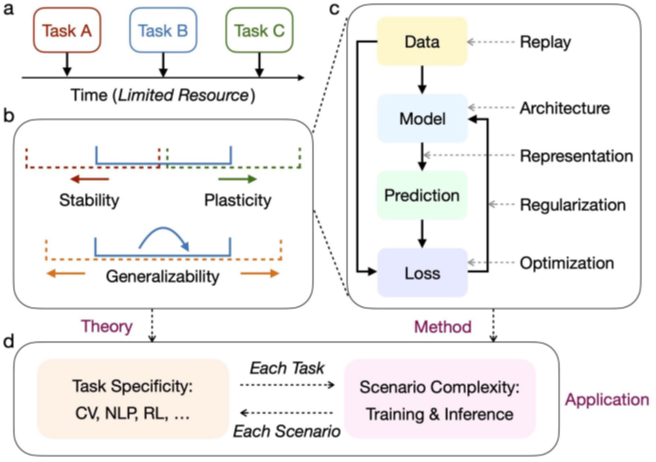
\includegraphics[width=0.5\textwidth]{imagenes/marco/Survey_of_Continual_Learning_fig1.png} % change path and filename
	\caption{Four key aspects of CL framework \cite{CL}.}
	\label{fig:cl_summary}
\end{figure}
